\mode<article>{\section{RTG-SLAM}} \mode<presentation>{\subsection{RTG-SLAM}}

\mode<article>{\subsection{Overview}}
\begin{frame}\mode<presentation>{\Frametitle{Overview}}
	\mode<presentation>{\blfootnote{\href{http://arxiv.org/abs/2404.19706}{(SIGGRAPH 2024) RTG-SLAM: Real-time 3D Reconstruction at Scale using Gaussian Splatting}}}
	\begin{figure}[htbp]
		\centering
		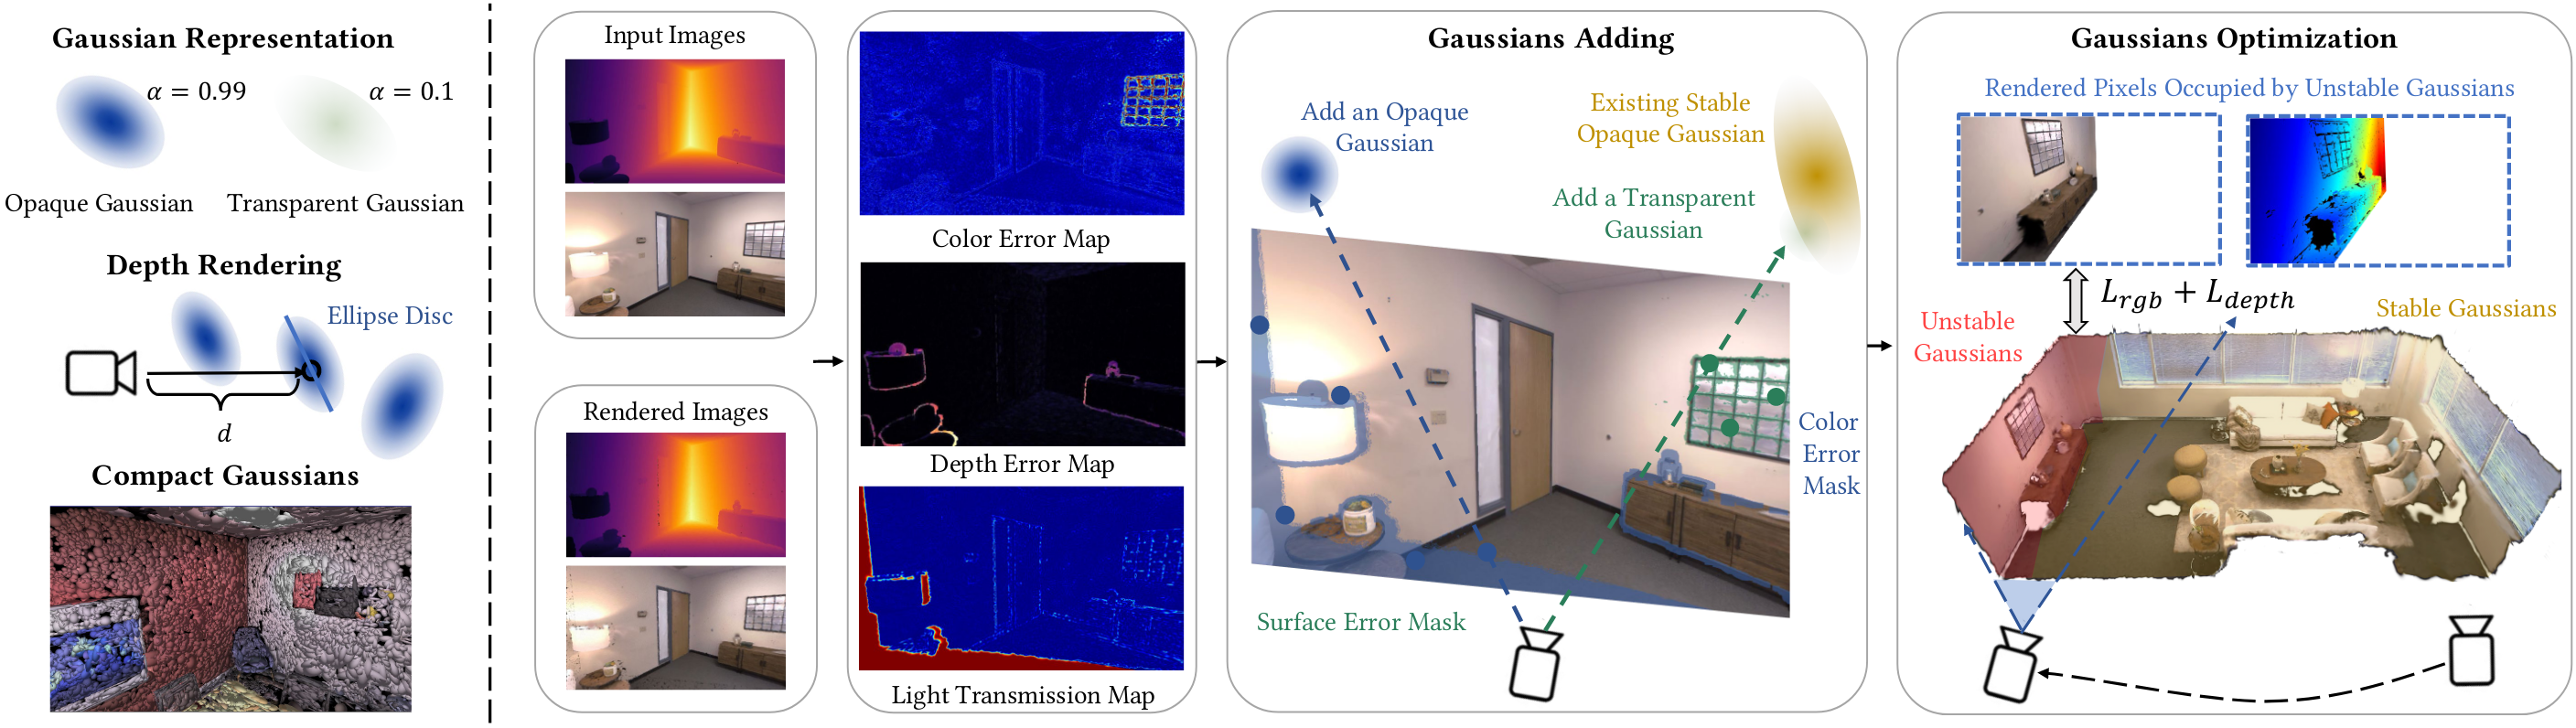
\includegraphics[width=\linewidth]{rtg-slam-overview.png}
		\caption{Overview of RTG-SLAM}
		\label{fig:rtg-slam-overview}
	\end{figure}
\end{frame}

\mode<article>{\subsection{Compact Gaussian Representation}}
\begin{frame}\mode<presentation>{\Frametitle{Compact Gaussian Representation \romannum{1}}}
	\mode<presentation>{\blfootnote{\href{http://arxiv.org/abs/2404.19706}{(SIGGRAPH 2024) RTG-SLAM: Real-time 3D Reconstruction at Scale using Gaussian Splatting}}}
	\mode<article>{
		\par The \alert{compact} 3D Gaussian-based scene representation in RTG-SLAM~\autocite{peng_rtg-slam_2024} can be denoted by equation~\ref{eq:rtg-slam-compact-gaussian}, where the colorful annotations are different from the original 3D Gaussian representation~\autocite{kerbl3Dgaussians}.
	}
	\begin{block}{Compact Gaussian Representation}
		\resetcolorseries[5]{marknode-color-series}
		\resetcolorseries[5]{annotation-color-series}
		\colorlet{marknode-convention}{Gray!20}
		\colorlet{annotation-convention}{Gray}
		\vspace*{1.5em}
		\begin{equation}
			\label{eq:rtg-slam-compact-gaussian}
			\tikzmarknode{n-convention-0}{\colorbox{marknode-convention}{\(\mathcal{S}\)}}  = \left\{ \mathcal{G}_i \vert i = 0,1,\cdots,N \right\}
			,\text{ where }
			\mathcal{G}_i = \left\{
			\tikzmarknode{n-convention-1}{\colorbox{marknode-convention}{\(\mathbf{x}\)}},
			\tikzmarknode{n-convention-2}{\colorbox{marknode-convention}{\(\mathbf{q}\)}},
			\tikzmarknode{n-convention-3}{\colorbox{marknode-convention}{\(\mathbf{s}\)}},
			\tikzmarknode{n-convention-4}{\colorbox{marknode-convention}{\(\mathbf{c}\)}},
			\tikzmarknode{n0}{\colorbox{marknode-color-series!![0]}{\(\alpha\)}},
			\tikzmarknode{n1}{\colorbox{marknode-color-series!![1]}{\(\mathbf{n}\)}},
			\tikzmarknode{n2}{\colorbox{marknode-color-series!![2]}{\(\eta\)}},
			\tikzmarknode{n3}{\colorbox{marknode-color-series!![3]}{\(t\)}}
			\right\}
		\end{equation}
		\begin{annotatedEquationEnv}
			\annotatedEquation{color}{n-convention-0}{north}{0em}{1.5em}{south west}{annotation-convention}{scene}{east}
			\annotatedEquation{color}{n-convention-1}{south}{0em}{-1em}{north east}{annotation-convention}{\(\in \mathbb{R}^3\), position}{west}
			\annotatedEquation{color}{n-convention-2}{south}{0em}{-2.5em}{north east}{annotation-convention}{\(\in \mathrm{SO}(3)\), rotation}{west}
			\annotatedEquation{color}{n-convention-3}{south}{0em}{-4em}{north east}{annotation-convention}{\(\in \mathbb{R}^3\), scale}{west}
			\annotatedEquation{color}{n-convention-4}{south}{0em}{-5.5em}{north east}{annotation-convention}{\(\in \mathbb{R}^{3n}\), color}{west}
			\annotatedEquation{colorseries}{n0}{south}{0em}{-7em}{north east}{annotation-color-series}{\(0.99\vee0.1\), ``boolean'' opacity}{west}
			\annotatedEquation{colorseries}{n1}{south}{0em}{-8.5em}{north east}{annotation-color-series}{\(\in \mathbb{R}^3\), normal vector}{west}
			\annotatedEquation{colorseries}{n2}{south}{0em}{-10em}{north east}{annotation-color-series}{confidence}{west}
			\annotatedEquation{colorseries}{n3}{south}{0em}{-11.5em}{north east}{annotation-color-series}{\(\in \mathbb{R}\), initialization timestamp}{west}
		\end{annotatedEquationEnv}
		\vspace*{11.5em}
	\end{block}
\end{frame}

\begin{frame}\mode<presentation>{\Frametitle{A Review of 3D Gaussian Splattings \romannum{1}}}
	\mode<presentation>{\blfootnote{\href{http://arxiv.org/abs/2404.19706}{(SIGGRAPH 2024) RTG-SLAM: Real-time 3D Reconstruction at Scale using Gaussian Splatting}}}
	\mode<article>{
		\par The appearance (RGB) rendering is basically the same as the original 3DGS. For the current frame, the Gaussians are sorted from front to back and re-indexed from \(0\) to \(N\), and then alpha-blending (equation~\ref{eq:alpha-blending}) is leveraged for image formation.
	}
	\begin{block}{\(\boldsymbol\alpha\)-blending\hfill Image Formation Model}
		\vspace*{6.5em}
		\resetcolorseries[6]{marknode-color-series}
		\resetcolorseries[6]{annotation-color-series}
		\begin{equation}\label{eq:alpha-blending}
			\tikzmarknode{n0}{\colorbox{marknode-color-series!![0]}{\(\hat{\mathbf{C}}\)}}
			(
			\tikzmarknode{n1}{\colorbox{marknode-color-series!![1]}{\(\mathbf{u}\)}}
			)
			=
			\sum_{
				i
				=0}^{
			\tikzmarknode{n2}{\colorbox{marknode-color-series!![2]}{\scriptsize \(N\)}}
			}
			\tikzmarknode{n3}{\colorbox{marknode-color-series!![3]}{\(\mathbf{c}_i\)}}
			\tikzmarknode{n4}{\colorbox{marknode-color-series!![4]}{\(p_i\)}}
			(\mathbf{u})
			\alpha_i
			\tikzmarknode{n5}{\colorbox{marknode-color-series!![5]}{\(\displaystyle \prod_{j=0}^{i-1} (1-p_j(\mathbf{u})\alpha_j)\)}}
		\end{equation}
		\begin{annotatedEquationEnv}
			\annotatedEquation{colorseries}{n0}{north}{0em}{6.5em}{south west}{annotation-color-series}{\(\mathbb{R}^{2} \mapsto \mathbb{R}^{3}\), the rendered RGB image}{east}
			\annotatedEquation{colorseries}{n1}{north}{0em}{5.5em}{south west}{annotation-color-series}{\(= \begin{bmatrix}
				h & w
			\end{bmatrix}^{\mathrm{T}}\), a pixel}{east}
			\annotatedEquation{colorseries}{n2}{north}{0em}{3em}{south west}{annotation-color-series}{the number of sorted and visible 3D Gaussians}{east}
			\annotatedEquation{colorseries}{n3}{south}{0em}{-4em}{north west}{annotation-color-series}{color of \(i\)-th Gaussian}{east}
			\annotatedEquation{colorseries}{n4}{south}{0em}{-1.5em}{north west}{annotation-color-series}{\(\mathbb{R}^{2} \mapsto [0,1]\), probability distribution of \\ \(i\)-th splatted(2D) Gaussian}{east}
			\annotatedEquation{colorseries}{n5}{north}{0em}{1em}{south west}{annotation-color-series}{\(T_i \in \mathbb{R}\), \\transmittance for \(i\)-th Gaussian}{east}
		\end{annotatedEquationEnv}
		\vspace*{4em}
	\end{block}
\end{frame}

\begin{frame}
	\mode<presentation>{\Frametitle{A Review of 3D Gaussian Splattings \romannum{2}}}
	\mode<presentation>{\blfootnote{\href{http://arxiv.org/abs/2404.19706}{(SIGGRAPH 2024) RTG-SLAM: Real-time 3D Reconstruction at Scale using Gaussian Splatting}}}
\end{frame}

